\chapter{Физико-математические задачи и вычислительные методы в исследованиях, проводимых с использованием высокопроизводительных ВС} \label{chapt2}
В последние годы (с 2010 по 2016 год) было опубликовано много статей (более 300) в различных международных журналах по тематике <<экзафлопсные вычисления>> (т.е. вычисления на перспективных суперЭВМ производительностью порядка $10^{18}$ операций с плавающей точкой в секунду), из них около трети посвящены решению различных прикладных задач.

В обзорную часть данной диссертационной работы вошло 298 статей.  Распределение статей по приложениям показано в таблице \ref{tab_physics}.

\begin{table}[ht]
	\caption{Распределение по приложениям статей относящихся к тематике <<экзафлопсные вычисления>>}
	\begin{center}
		\begin{tabular}{|c|c|}
			\hline
			вычислительная гидродинамика & 27  \\ \hline 
			ядерные технологии & 17       \\ \hline  
			физика плазмы & 11  \\ \hline 
			разработка новых материалов & 10  \\ \hline 
			предсказание погоды & 10 \\ \hline 
			биомедицинские приложения & 9 \\ \hline 
			астрофизика и космология & 6  \\ \hline 
			молекулярная динамика   & 6   \\ \hline 
			мультифизика & 6              \\ \hline 
			геофизика & 6  \\ \hline 
			финансы & 2  \\ \hline 
		\end{tabular}
	\end{center}
	\label{tab_physics}
\end{table}

Как видно из таблицы \ref{tab_physics} особенно активно математическое моделирование используется в следующих областях науки и техники.  
\begin{itemize}
	\item Гидродинамика (космическая газодинамика, расчет обтекания кораблей и самолетов, например, из числа статей, относящихся к пета- и экзафопсным вычислениям, \cite{Onishi2014},\cite{Lu2015,Peterson1989}, предсказание наводнений в прибрежных городах Северной Европы и другие экологические вопросы, моделирование океанических течений \cite{STERN20151,Newman20152086,Reuter2015325,Walker2014287}, расчет гидродинамической турбулентности %\cite{BirdsallIEEE}%
	\cite{Mininni2011316,Appeloe201019,Yokota2013445,Tucker2016,Kotov2016189}  моделирование многофазных течений \cite{Safi2016170,Zaspel2016505}, построение сеток для гидродинамического моделирования \cite{Shang2013381,Yilmaz2013388,Ono20142336,Yilmaz2013773}),
	\item Ядерные технологии, точнее моделирование различных процессов, протекающих в ядерных реакторах. \cite{Romano2013274,Romano201320,Romano201590,Boyd201443,Gong2012588,Gong20116010,Bergmann2015176,Bauge201432}, 
	\item Разработка новых материалов (квантовохимические расчеты структуры и поведения молекул, вычисление супер-многомерных интегралов в различных приближениях \cite{Ono2015}), методы молекулярной динамики \cite{Valiev20101477,Aguilar20132197,Yokota201317,Ohno20142575,Xu2015200}
	\item Моделирование ускорителей заряженных частиц \cite{Silva2014229}, 
	\item Плазменные технологии\cite{BirdsallIEEE}
	\item Плазменные процессы в установках управляемого термоядерного синтеза
	\cite{KatesHarbeck2016231,Winkel2015456,Minoshima201381,Kumar20132251,Decyk2014,Acebron2013224}. 
	\item Разработка новых лекарств и другие биомедицинские приложения \cite{Stone2015,Joshi2011200,Saraladevi2015596,Blau20132856,Wang2012254,Markram201139,Markowitz2015730} (наибольшее количество расчетов с использованием большого количества процессоров, производилось именно в этой области). 
	
	\item Также математические модели для пета-и экзафлопсных суперЭВМ создаются в геофизике \cite{Christen2012956,Nakajima20131265,Zhong2015197,Reed20131,Hodges201316,Furumura20111448}.
\end{itemize}

С учетом того, что во многих областях приходится иметь дело с несколькими различными и одновременно протекающими физическими процессами при этом эти различные процессы моделируются совершенно различными способами, существует необходимость разработки высокомасштабируемого программного обеспечения для таких приложений, которые в зарубежной литературе называются мультифизическими (multiphysics). Это делается в работах \cite{Yamamoto2014576,Agullo201196,Ettrich20151,Vazquez2016,
	Liu2011261,Zheng2015313}.

Наиболее существенной областью приложений пета- и экзафлопсных вычислений оказались ядерные технологии и вопросы моделирования ядерных реакторов (статей, посвященных вычислительной гидродинамике, больше, как видно из таблицы \ref{tab_physics}, но это очень обширная и разнообразная область). В основном разрабатываются масштабируемые версии методов Монте-Карло для переноса нейтронов \cite{Romano2013274,Romano201320,Romano201590,Boyd201443,Gong2012588,Gong20116010,Bergmann2015176,Bauge201432}, проводится анализ коммуникационных потерь в методе Монте-Карло \cite{Siegel20123119,Horelik2014646,Tramm2016}. Также рассматриваются вопросы взаимодействия пучков частиц с материалами \cite{Bandura20103485} и применение решеточных уравнений Больцмана с использованием квантовой хромодинамики к задачам ядерной физики\cite{Beane20111,Savage2012140}.
Следует особенно отметить работы по созданию интегральной среды для разработки ядерных реакторов \cite{Patterson201697} и моделирование новых видов реакторного топлива \cite{Stan200920}.

Разработка технологии решения физических задач с помощью современных и перспективных высокопроизводительных ЭВМ составляет содержание диссертационной работы. Использование суперЭВМ будет показано на примере решения задач динамики плазмы, аналогичных, рассмотренным в \cite{BretPoP2010,BirdsallIEEE,LangdonBirdsall}. Эти задачи представляют чрезвычайно большой научный интерес, а также очень актуальны с точки зрения использования результатов моделирования в промышленности. Такой выбор не ограничивает общности полученных в данной работе результатов, так как разработанные суперкомпьютерные технологии могут быть применены также и в других областях, в особенности в гидродинамическом и в квантовохимическом моделировании.

В частности, одной из важных областей приложения созданных методов оказывается сейсмология, при использовании метода частиц
\cite{hockney,VshivkovPICbook} как альтернативы решению уравнения эйконала \cite{Engquist}.

%Плазменные задачи представляют большой интерес как с точки зрения выбора и обоснования модели (равновесная плазма или неравновесная, устойчивая или неустойчивая, магнитогидродинамическое описание или кинетика), так и с точки зрения  вычислительных методов (решение уравнения Пуассона или уравнений Максвелла, выбор одного из многих вариантов решения кинетического уравнения или уравнений МГД), и в особенности с точки зрения разработки и программной реализации вычислительных алгоритмов (различные варианты декомпозиции расчетной области, организации межпроцессорных обменов, достижения оптимальной производительности), т.е. плазменные задачи требуют поиска новых решений на всех уровнях триады Академика А.А.Самарского: <<модель, алгоритм, программа>> \cite{SamarskiMatMod}.  

%Все перечисленные вопросы в том или ином виде встречаются и в других областях математического моделирования, тем не менее в физике плазмы есть проблемы, не имеющие аналога по степени сложности (и соответственно, по количеству необходимых для решения вычислительных ресурсов). Эти проблемы возникают при моделировании плазменных неустойчивостей и турбулентностей в установках управляемого термоядерного синтеза (УТС) при высоких температурах (1-5 КэВ, что соответствует 10 млн.градусов), когда плазма не является даже приближенно равновесной в сколь угодно малой окрестности. В этом случае плазма имеет очень большое количество степеней свободы \cite{MohographyKhoroshevsky}, необходимость учета которых приводит к использованию соответствующих больших объемов памяти.

%Особенная важность решения задачи о динамике плазмы в установках УТС связана с тем, что управляемый термоядерный синтез является единственным вариантом решения энергетической проблемы. Все существующие альтернативные энергетические концепции имеют очень серьезные недостатки, не позволяющие рассматривать их как решение энергетической проблемы в мировом масштабе: углеводородная энергетика имеет ограниченные запасы топлива, атомная энергетика представляется экологически опасной, электростанции на солнечной энергии не могут строится из-за (возможно, временной) дороговизны и экологических проблем, возникающих при производстве фотоэлементов в больших количествах, а различного рода <<экологически чистые>> электростанции, такие как ветряные, приливные, геотермальные не могут строится в необходимых больших количествах, также, как и крупные ГЭС.

%Другая важная область приложения моделирования плазмы - это промышленные плазменные технологии, используемые, в частности, для производства чистого кремния для нужд микроэлектронной промышленности и для производства микропроцессоров (установки молекулярно-лучевой эпитаксии). Также моделирование высокотемпературной плазмы может быть полезно для исследования природы солнечных вспышек и исследования их влияния на магнитосферу Земли и арктическую навигацию \cite{RussellIEEE}.

%Подводя предварительный итог, нужно подчеркнуть еще раз, что применение современных высокопроизводительных ЭВМ может дать качественный скачок в решении многих важных научных и производственных задач. Далее необходимо дать краткое описание этих ЭВМ с тем, чтобы определить стратегию их использования в интересах математического моделирования. 

%На недавних суперкомьютерных конференциях \cite{Abrau2011} широко обсуждались вопросы связанные с построением экзафлопс-компьютеров и трудностями создания программного обеспечения для них. 
%В первую очередь это чрезвычайно большое ожидаемое энергопотребление - порядка 1 ГВт. Таким образом, на первый план выходят вопросы эффективной эксплуатации такой исключительно дорогой машины, а энергоэффективность алгоритма становится определяющей чертой для допуска этого алгоритма к расчетам.

%Ограничивая суперкомпьютерный мир первой десяткой наиболее мощных компьютеров мира, а это вполне оправдано в том случае, если речь идет о возможной архитектуре экзафлопс-компьютера,  можно сказать, что этот мир весьма неоднороден. Серьезно отличаются базовые элементы, на основе которых строятся суперЭВМ , как процессоры (Intel Xeon, AMD Opteron, Sun UltraSPARC), так и ускорители вычислений (Intel Xeon Phi, Nvidia Kepler). 

%С учетом того, что наиболее мощные компьютеры строятся ( вероятнее всего и дальше будут строиться \cite{Lu2015}) на основе ускорителей вычислений \cite{Stepanenko2010}, для эффективного использования компьютеров большой мощности с целью решения актуальных физических задач принципиально необходимо значительно упростить освоение гибридных (т.е. построенных с использованием как процессоров общего назначения, так и ускорителей вычислений) суперЭВМ с точки зрения специалиста по моделированию в конкретной предметной области или физика. 
%Описанное разнообразие архитектур означает, что все реализации вычислительных алгоритмов для перспективных экзафлопс-компьютеров должны быть в достаточной степени универсальными, чтобы иметь возможность проводить расчеты на тех процессорах или ускорителях вычислений, которые будут  выбраны для создания экзафлопс-компьютера, в частности, на всех перечисленных типах вычислительных устройств. 


%Кроме того, следует отметить широко обсуждаемые трудности создания программного обеспечения для экзафлопсных суперЭВМ, связанные с наличием в составе этих суперЭВМ сотен тысяч и миллионов процессорных элементов. По данному вопросу существует две противоположных точки зрения. 
%Согласно одной из них, для эффективной работы на экзафлопсных суперЭВМ потребуется создание принципиально новых математических основ вычислительной техники, операционных систем, языков программирования и пр., не требующих межпроцессорных коммуникаций в принципе. Другая точка зрения заключается в том, что решение задач на экзафлопсных суперЭВМ будет производится с использованием существующего программного обеспечения, т.е коммуникационных библиотек, основанных на сообщениях \cite{Gropp2009} и алгоритмических языках программирования. 

%Таким образом, можно строить реализацию вычислительных алгоритмов для 
%экзафлопсных суперЭВМ на основе модели передачи сообщений (самый известный ее вариант называется MPI) и исходя из предположений об иерархической структуре коммуникационной системы.
%Наиболее важным вопросом реализации вычислительного алгоритма на суперЭВМ является вопрос масштабируемости алгоритма, то есть обеспечение равномерной загрузки процессорных элементов - отдельных процессоров, ускорителей вычислений или узлов суперкомпьютера.  Это один из вопросов, для которых в настоящей работе предложено эффективное решение.

%Одним из наиболее эффективных принципиальных подходов к созданию эффективных параллельных алгоритмов является сборочная технология параллельного программирования \cite{MalyshkinSynthesis,MalyshkinASSY,Kraeva2001,
%	MalyshkinTsigulin}, согласно которой параллельная программа собирается из множества   готовых атомарных фрагментов, содержащих как данные, так и алгоритмы.

%Существует множество подходов, используемых для достижения более высокой производительности, 
%\begin{itemize}
%	\item декомпозиция расчетной области\cite{Liewer1989,Kraeva2001,Stijnman2003, Eastwood1995}, с целью ее разделения на более мелкие подобласти, 
%	\item использование большого количества процессорных элементов (разработка системного программного обеспечения, позволяющего увеличить число ПЭ сверх определенного предела
%	\cite{Gropp2009} или создание численных методов с меньшим количеством необходимых коммуникаций)
	%\item применение многоядерных процессоров или различных ускорителей вычислений \cite{SteYuz13}. позволяющих увеличить скорость счета без возрастания нагрузки на коммуникационную сеть, оптимизация под архитектуру процессора или ускорителя, 
	%\item сокращение количества отправляемых сообщений, 
	%\item переход к численным методам, более подходящим для многопроцессорных ЭВМ (от неявных схем к явным, к методам на основе ортогональных преобразований. от методов, рассматривающих объект моделирования как сплошную среду к методам частиц и пр.) или численных методов специально подобранных или специально оптимизированных для решения конкретной задачи. 
%\end{itemize}

%Однако все перечисленные подходы можно разделить на три принципиально разных непересекающихся направления:
%\begin{itemize}
%	\item увеличение числа ПЭ
%	\item адаптация вычислительных методов к архитектуре суперЭВМ
%	\item использование ускорителей вычислений 
%\end{itemize}

%С этой точки зрения был проведен обзор недавних (2010-2016 годы) публикаций, относящихся к тематике <<экзафлопсные вычисления>> в журналах Future Generation Computer Systems, Procedia Computers Science, Journal of Parallel and Distributed Computing, Parallel Computing, Journal of Computational Physics, Computer Physics Communications и др.
%По трем указанным выше направлениям они распределились, как показано на рисунке \ref{exaflops_topics_fig}.

% \begin{center}
% 	\begin{figure}[htb]
% 		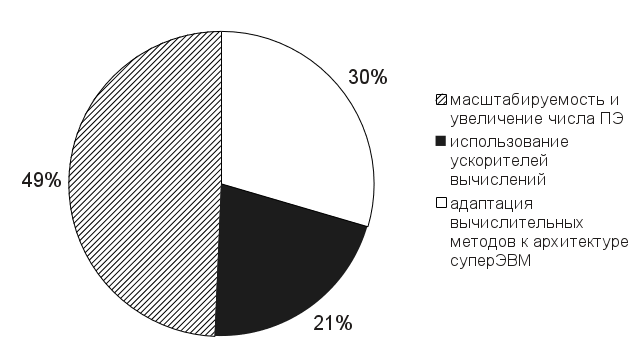
\includegraphics[height=7cm,keepaspectratio]{images/exaflops_topics.png}
% 		\caption{Распределение по направлениям статей относящихся к тематике <<экзафлопсные вычисления>>}
% 		\label{exaflops_topics_fig}
% 	\end{figure}
% \end{center}




%\begin{table}[ht]
%\caption{Распределение по направлениям статей относящихся к тематике <<экзафлопсные вычисления>>}
%\begin{center}
%\begin{tabular}{|c|c|c|}
%\hline
%Условное наименование направления      & Число статей & В \%  от     \\
%                                       &              & общего числа \\ \hline
%масштабируемость и увеличение числа ПЭ & 147 &          49 \\  \hline
%использование ускорителей вычислений   & 63  &          21 \\  \hline
%адаптация вычислительных методов к архитектуре суперЭВМ
%  & 88  &          30       \\ \hline  
%\end{tabular}
%\end{center}
%\label{exaflops_topics_tab}
%\end{table}

% \begin{table}[ht]
% 	\caption{Распределение по темам статей относящихся к направлению
% 		<<масштабируемость и увеличение числа ПЭ>>}
% 	\begin{center}
% 		\begin{tabular}{|c|c|c|}
% 			\hline
% 			Тема                       & Количество          & В \%           \\
% 			& статей в обзоре     & от общего числа  \\ \hline 
% 			масштабируемые                 & 29 & 9.73  \\    
% 			архитектуры                    &    &       \\   \hline
% 			программные средства           &    &       \\
% 			для повышения                  &    &       \\
% 			масштабируемости              & 18 & 6.04  \\ \hline 
% 			Ускорители и                   &    &      \\
% 			специальное оборудование       &    &      \\
% 			для повышения                  &    &      \\
% 			масштабируемости              & 16 &  5.37 \\ \hline 
% 			Моделирование                  &    &     \\
% 			функционирования               &    &     \\
% 			экзафлопсных систем            & 19 & 6.38  \\ \hline 
% 			Упрощение работы с             &    &          \\
% 			экзафлопсными системами       & 11 & 3.69 \\ \hline 
% 			Декомпозиция                   &    &	      \\
% 			расчетной области             & 10 &  3.36 \\ \hline 
% 			Динамическая                   &    &       \\
% 			балансировка загрузки          & 24 &  8.05 \\ \hline 
% 			Отказоустойчивость             & 20 & 6.71  \\ \hline 
% 			Уменьшение                     &    &        \\
% 			количества коммуникаций        & 10 & 3.36   \\ \hline 
% 		\end{tabular}
% 	\end{center}
% 	\label{topic_maxPE}
% \end{table}
% \textbf{Первое направление}, названное условно <<масштабируемость и увеличение числа ПЭ>> было, в свою очередь, разделено
% на несколько тем, как показано в таблице \ref{topic_maxPE}. 
% \clearpage
% 
% К теме <<масштабируемые архитектуры>> были отнесены такие работы, как, например, алгоритм привязки процессов к узлам на коммуникационной сети суперЭВМ в виде трехмерного тора \cite{Kodama2014362},
% метаматематические основы проектирования бесконечно расширяемых машин на основе идеальной модельной архитектуры \cite{Anderson20151828}, опыт эксплуатации и решения задач на машине K computer (№ 4 в списке Top500 за ноябрь 2015), имеющей хорошие характеристики масштабируемости и, в отличие от № 1 и № 2, построенной не на основе ускорителей вычислений \cite{Yamamoto2014576}. Также к этой теме отнесена работа, посвященная использованию большого количества ядер в программах, написанных для старых компьютерных архитектур: несмотря на то, что работа посвящена программированию, основные вопросы, которые там решаются - это архитектурные вопросы, точнее преодоление архитектурных различий программными средствами \cite{Lohner201353}.
% 
% К теме <<программные средства для повышения масштабируемости>> отнесены разработки коммуникационного программного обеспечения, например, MPI, специально предназначенного для работы с очень большим количеством процессов \cite{Zounmevo2014265}, или механизмы снижения задержки сообщений в MPI \cite{Khunjush2009430}. Также к этой теме относится создание высокомасштабируемых пакетов программ для решения конкретных задач \cite{Valiev20101477,Peng20131469}.
% 
% Следующая тема, <<Ускорители и специальное оборудование для повышения масштабируемости>>, образована такими работами, как исследование масштабируемого ввода-вывода на кластере из ПЛИС \cite{Schmidt2012344}. Следует отметить, что к этой теме не относятся вопросы конструирования кластеров на ПЛИС и соответствующие проблемы программирования, а только лишь влияние необычного оборудования (в частности ПЛИС) на масштабируемость. Кроме того, к этой теме отнесены исследование поведения закона Амдала \cite{Amdahl} на многоядерных системах \cite{Yavits2014} и разработка специализированного сетевого оборудования типа <<сеть на кристалле>>  \cite{Khanjari2015403}, а также создание
% сопроцессоров для диспетчеризации потоков \cite{Giorgi2015100}.
% 
% В связи с отсутствием реально функционирующих суперЭВМ экзафлопсного класса, а также в связи с предполагаемой исключительной дороговизной вычислительного времени на этих системах, особенную важность приобретает тема  <<Моделирование функционирования экзафлопсных систем>>, включающая в себя также	 и моделирование работы прикладных программ на этих системах. К этой теме относятся анализ расхода времени на коммуникации \cite{Siegel20123119} и подбор с помощью моделирования оптимального (по коммуникациям) варианта декомпозиции расчетной области \cite{Hag2015400}, а также моделирование и предсказание аварийных ситуаций \cite{Aupy20142048}.
% 
% 
% 
% В докладе профессора Н.Н.Миренкова на конференции Parallel Computing Technologies-2009 (PaCT-2009) \cite{Watanobe2009} была высказана точка зрения о том, что на новые поколения суперЭВМ (гигафлопсные, терафлопсные, петафлопсные,...) раз за разом возлагались очень серьезные надежды на прогресс в решении реальных физических задач, тем не менее реальные успехи могут быть охарактеризованы лишь как очень скромные. Причина этого, по мнению Н.Н.Миренкова \cite{Watanobe2009} заключается в том, что специалисты в конкретной предметной области не понимают, как можно использовать суперЭВМ, и не видят смысла в их использовании. Возможный выход заключается в создании удобных, интуитивно понятных инструментов для создания программ на суперЭВМ. Такие работы активно ведутся, и в рамках настоящего обзора они выделены в тему <<Упрощение работы с  экзафлопсными системами>>. Сюда относятся создание учебников по конструированию и эксплуатации кластеров \cite{Georgi20111917}, разработка средств отладки параллельных приложений \cite{Jin20131774,Huenich20151383}, а также создание новых средств администрирования \cite{Gallard2012136}.
% 
% Важнейшим вопросом для обеспечения высокой масштабируемости при решении конкретных задач является декомпозиция расчетной области. К этой теме отнесены работы, в которых основное внимание уделяется изначальному распределению загрузки, т.е. без динамики, а также те работы, в которых предлагается оптимизация доступа к данным независимо от их распределения в рамках вычислительной системы \cite{Srinivasa2012256,Lieb2014246}, или разрешение конфликтов при распределении различных видов данных, с различными вариантами доступа к ним, например, \cite{Sitaraman2016,Balzuweit201667}.
% 
% В отличие от предыдущего пункта, к теме <<Динамическая балансировка загрузки>> отнесены вопросы оптимизации загрузки процессорных элементов, проводимой во время работы программы, например, исследование воздействия несбалансированности загрузки на производительность методов Монте-Карло \cite{Siegel2013901} или реализация метода частиц в ячейках с динамической балансировкой загрузки на языке parallel C \cite{Verleye201310}, а также вопросы, связанные с балансировкой загрузки не только прикладной программы, но и вычислительной системы в целом, что особенно важно с точки зрения перспективы экзафлопсных вычислений \cite{Dong20121254}.
% 
% 
% 
% Следующая тема, <<отказоустойчивость>>, исключительно важна для подготовки к вычислениям на экзафлопсных машинах,
% с учетом того, что различного сорта ошибки будут происходит на системах, состоящих из миллионов процессоров практически каждую секунду. Кроме того, стоимость проведения таких расчетов, как ожидается, будет очень высокой (сейчас расчет продолжительностью в 10 млн. процессоро-часов с использованием метода частиц в ячейках оценивается в 0.5 млн. евро \cite{Vieira}). К этой теме относятся
% обработка контрольных точек, оптимизация и ускорение их чтения и записи \cite{Nicolae2013698,Casanova20157}, диспетчеризация процессов с учетом наличия поврежденных или вышедших из строя процессорных элементов \cite{Defour20161},
% а также анализ производительности реализации MPI, работающей с учетом наличия в системе сбоев \cite{Hursey201215}.
% 
% К последней теме (<<уменьшение количества коммуникаций>>) в рамках направления <<масштабируемость и увеличение числа ПЭ>> отнесены статьи, посвященные созданию параллельных алгоритмов, стремящихся к минимуму коммуникаций (англ. communication-avoiding \cite{Dongarra2013212}). Важность этой темы очевидна для экзафлопсных вычислений: при наличии миллионов процессорных элементов, обменивающихся сообщениями, количество сообщений оценивается (минимально), как $O(N)$, где $N$ - число процессоров, поэтому очень важна разработка алгоритмов, способных или вовсе обойтись без коммуникаций или снизить их количество до $O(1)$. К таким алгоритмам относятся: метод решёточных уравнений Больцмана \cite{Wittmann2013924,Safi2016170}, а также, разработка модели свободной поверхности океана с минимизацией объема коммуникаций\cite{Newman2016877} или решение уравнений типа уравнения Пуассона алгебраическим многосеточным методом, масштабируемым в том смысле, что время решения пропорционально количеству неизвестных (а не количеству ПЭ) \cite{Notay2015237}.
% 
% 
% 
% \textbf{Второе направление} работ над экзафлопсными вычислениями, выделенное в рамках обзора, названо <<адаптация вычислительных методов к архитектуре суперЭВМ>>. 
% 
% Сюда относятся численные методы, разработанные специально для экзафлопсных машин (методика локального сгущения шага при решении уравнений реакции-диффузии \cite{Krause2016164}, решение дифференциальных уравнений в частных производных с пониженным объемом коммуникаций \cite{Norman2015}).
% Другая тема  - адаптация имеющихся численных методов для работы на очень большом количестве ПЭ (например, вариант итерационного метода Якоби с ускорением Андерсона \cite{Pratapa201643} или масштабируемые алгоритмы Монте-Карло для финансового моделирования \cite{Alexandrov20111708}). Здесь необходимо ответить на вопрос: где проходить грань между алгоритмами, специально разработанными для экзафлопсных машин, и алгоритмами, адаптированными для экзафлопса. Казалось бы, разница незначительна, и более того, поскольку то, что разрабатывается специально для экзафлопсных суперЭВМ, также разрабатывается не на ровном месте, то можно сказать, что разницы нет вовсе, что это просто одно и то же. Тем не менее  разница здесь фундаментальна, разница та же, что между свойством и определением. Алгоритмы, разработанные специально для экзафлопсных вычислений - это те алгоритмы, разработка которых изначально проводилась с целью минимизировать или свести к нулю коммуникации и обеспечить высокую энергоэффективность  (с достижением физической корректности результатов). С другой стороны, алгоритмы к экзафлопсным вычислениям адаптированные -  это те алгоритмы, которые разрабатывались для параллельных вычислений на десятках или сотнях ПЭ, и которые случайно оказались достаточно хорошо масштабируемыми для их эксплуатации на пета- и экзафлопсных системах. Фундаментальный характер имеющихся различий заключается еще и в том, 
% что энергоэффективными эти алгоритмы почти никогда оказаться не могут по той причине, что разрабатывались они для процессоров общего назначения, и изменить это в процессе адаптации невозможно без принципиальных изменений самого алгоритма.
% 
% Также к направлению <<адаптация вычислительных методов к архитектуре суперЭВМ>> отнесены статьи, посвященные работе с данными большого размера. Это один из важнейших вопросов при подготовке к счету на экзафлопсных суперЭВМ, вызванный очевидной необходимостью сохранить результаты счета объемом в сотни петабайт \cite{Abramson20141} и передавать их для обработки. Разделение направления по темам показано в таблице \ref{topic_special}.	
% 
% Под названием темы <<со-дизайн и комплексная разработка программ>> подразумеваются подходы к разработке параллельных 
% вычислительных приложений с учетом особенностей вычислительной системы \cite{Poghosyan2015167}, 
% многоуровневый параллелизм \cite{Jacobsen20131,Liu2011261}, реализация параллельного алгоритма с учетом особенностей решаемой физической задачи \cite{Rycerz20131116}, 
% сочетанием различных подходов к параллельной реализации \cite{Chakroun20131563,Jin2011562} и др.      
% В работе \cite{Emad2016} представлен подход, названный <<объединяй и властвуй>>, который заключается в следующем: параллельная программа, реализующая некоторую математическую модель, разбивается на три элемента, а именно вычисления, работу с данными и коммуникации. При этом все три элемента тесно взаимодействуют между собой, но  разрабатываются различным образом и могут быть представлены каждый несколькими компонентами, что обеспечивает адаптацию к структуре суперЭВМ и выбор оптимальных численных методов. 
% В статье \cite{Dosanjh2014} излагаются различные возможные подходы аппаратной точки зрения к построению экзафлопсного суперкомпьютера с  на примере нескольких действующих машин-прототипов с аналогичной архитектурой, но меньшей мощности. Моделирование расчетов на экзафлопсных системах проводится на машинах-прототипах с помощью так называемых мини-приложений. 
% В работе \cite{Subotic2013450} разработана методoлогия упрощения создания и улучшения переносимости приложений для экзафлопсных суперЭВМ, которая называется <<разработка сверху вниз>> (top down methodology). Данная методология основывается на следующем: разработка кода проводится так, чтобы он не был привязан к типу параллелизма или используемому оборудованию. Доработка под реально имеющееся оборудование  проводится на следующей стадии разработки и таким образом код может быть перенесен и запущен на любом типе суперЭВМ.
% 
% 
% 
% 
% \begin{table}[ht]
% 	\caption{Распределение по темам статей относящихся к направлению
% 		<<адаптация вычислительных методов к архитектуре суперЭВМ>>}
% 	\begin{center}
% 		\begin{tabular}{|c|c|c|}
% 			\hline
% 			Тема                       & Количество          & В \%           \\
% 			& статей в обзоре     & от общего числа  \\ \hline 
% 			адаптация вычислительных методов   &   & \\
% 			к экзафлопсу                       & 19 & 6.38  \\ \hline 
% 			Вычислительные методы, специально & & \\
% 			разработанные для экзафлопса & 17 & 5.70 \\ \hline 
% 			Обработка данных  & & \\
% 			большого размера  & 30 & 10.07 \\ \hline 
% 			Со-дизайн и комплексная        &    &     \\      
% 			разработка программы           & 13 & 4.36   \\  \hline 
% 			
% 		\end{tabular}
% 	\end{center}
% 	\label{topic_special}
% \end{table}
% 
% \clearpage
% 
% \textbf{Третье направление} работ над экзафлопсными вычислениями, названное условно <<использование ускорителей вычислений>>, было также разделено на несколько тем, как показано в таблице \ref{topic_GPU}.
% 
% Наиболее очевидное применение ускорителей - ускорение расчетов (первая строка в таблице \ref{topic_GPU}), например, вопрос о том, как получить на методе частиц в ячейках заявленную для ускорителя Intel Xeon Phi производительность в 1 Teraflops \cite{Nakashima2015}, или расчеты в области микроволновой томографии для обнаружения рака груди с использованием процессоров IBM Cell \cite{Xu20121106}. Также рассматриваются затруднения, возникающие при работе с памятью при реализации методов Монте-Карло на многоядерных системах \cite{Tramm2015195}, и проблемы эффективной реализации метода частиц в ячейках на GPU \cite{Gong2012588,Kong2011,Safi20151290}.
% 
% Несмотря на то, что использование ускорителей вычислений, как графических, так и Intel Xeon Phi и ПЛИС, обещает
% очень серьезные преимущества как по производительности, так и по энергоэффективности, реализация вычислительных алгоритмов на  ускорителях остается очень сложным вопросом по сравнению с реализацией их на процессорах общего назначения. В связи с этим актуальной является тема <<упрощение использования ускорителей>>.
% В частности, предложен набор программных инструментов для упрощения разработки \cite{Dongarra2015}.
% Кроме того, рассматриваются вопросы переноса программ между различными ускорителями вычислений \cite{Subotic2013} и 
% создание настраиваемых алгоритмов для GPU на примере метода частиц \cite{Decyk2011}. 	 
% 
% Следующая тема названа <<новые типы ускорителей>>. При формулировке такой темы этом необходимо ответить на вопрос, какие ускорители вычислений, и почему считаются новыми. В настоящее время для построения суперЭВМ в основном используются в основном два типа ускорителей: ускорители Intel Xeon Phi и графические ускорители Nvidia Kepler и Nvidia Tesla. Несмотря на то, что и ПЛИС, и графические ускорители корпорации AMD (например, AMD Firestream), и многоядерный процессор IBM Cell существуют достаточно давно, они используются значительно реже. Это дает определенные основания считать все эти ускорители, кроме 
% Intel Xeon Phi, а также Nvidia Kepler и Nvidia Tesla новыми (или нетрадиционными) типами ускорителей вычислений. К этой теме отнесено сравнение высокоуровневых инструментов реализации численных алгоритмов на ПЛИС \cite{Warne201495} и опыт создания и эксплуатации кластера на процессорах ARM с пониженным энергoпотреблением \cite{Rajovic2014}. Следует особенно отметить, что последняя работа посвящена именно вычислениям на таком кластере и проблемам достижения вычислительной производительности.
% 
% \begin{table}[ht]
% 	\caption{Распределение по темам статей, относящихся к направлению
% 		<<использование ускорителей вычислений>>}
% 	\begin{center}
% 		\begin{tabular}{|c|c|c|}
% 			\hline
% 			Тема                       & Количество          & В \%           \\
% 			& статей в обзоре     & от общего числа  \\ \hline 
% 			
% 			ускорение расчетов    &    &       \\ 
% 			с помощью ускорителей & 16 & 5.37  \\ \hline 
% 			упрощение использования  & & \\
% 			ускорителей & 8  & 2.68   \\ \hline 
% 			новые типы ускорителей & 8 & 2.68    \\ \hline 
% 			энергоэффективность &  31  & 10.40     \\ \hline 
% 		\end{tabular}
% 	\end{center}
% 	\label{topic_GPU}
% \end{table}
% 
% Естественным образом отсюда можно перейти к следующей теме: <<энергоэффективность>>. Эта тема особенно важна для экзафлопсных вычислений, в силу того что если суперЭВМ будут строится также, как сейчас, то экзафлопсный суперкомпьютер будет иметь слишком высокое энергопотребление. Это можно проиллюстрировать следующим образом: производительность 2-го по мощности компьютера в мире (Tianhe-2) в 30 раз меньше, чем 1 экзафлопс, однако если его энергопотребление (17.8 МВт) умножить на 30, получится 534 МВт, превышающее мощность большинства ядерных реакторов. 
% Аналогично для суперкомпьютера № 1, Sunway TaihuLight, эти показатели составляют 125 Петафлопс и 15 МВт соответственно. Разница с экзафлопсом в 8 раз, оценочное энергопотребление такой системы с экзафлопсной производительностью 120 МВт, что значительно меньше, но тем не менее, очень много, при том, что базовые элементы суперкомпьютера Sunway TaihuLight пока не используются массово при производстве суперЭВМ - поэтому ориентриваться на них, т.е. на процессоры Sunway SW26010 260C при прогнозировании перспективных 
% архитертур суперЭВМ нельзя.
% 
% Так или иначе это означает необходимость радикального понижения энергопотребления суперЭВМ. К теме <<энергоэффективность>> в рамках настоящего обзора отнесены следующие работы: исследование производительности методов Монте-Карло с учетом энергопотребления \cite{Atanassov20152719}, методы измерения, моделирования и управления энергопотреблением \cite{Goel20127} и стратегия создания энергоэффективных программ \cite{Trefethen2013}. 
% 
% 
% 
% 
% 
% Таким образом, по материалам обзора можно сказать, что наиболее актуальными вопросами с точки зрения экзафлопсных вычислений являются энергоэффективность (10.4 \% статей в обзоре, таблица \ref{topic_GPU}),
% обработка данных большого размера (10.07 \% статей, таблица \ref{topic_special}) и  разработка масштабируемых суперкомпьютерных архитектур (9.73 \% статей, таблица \ref{topic_maxPE}).
% 
% С другой стороны недостаточное внимание по результатам обзора в научной литературе, по крайней мере в рассмотренных журналах, уделяется созданию вычислительных методов специально предназначенных для экзафлопсных суперЭВМ (5.7 \% в таблице \ref{topic_special}), и даже вопросам адаптации вычислительных методов к экзафлопсным вычислительным системам (там же, 6.38 \%). Более того, в основном рассматриваются варианты методов Монте-Карло и методы решения больших СЛАУ, преимущественно на основе методов подпространства Крылова. Остальные методы и технологии математического моделирования в применении к экзафлопсным суперЭВМ изучаются значительно реже.
% 
% Также сравнительно небольшое внимание (4.36 \%, таблица \ref{topic_special}) уделяется такому важному вопросу как со-дизайн  и комплексная разработка программ. При этом важно отметить, что лишь две работы из представленного списка (\cite{Emad2016,Subotic2013450}) используют подход со-дизайна полностью, остальные ограничиваются лишь отдельными его элементами, в частности, не производится переработка самого численного метода под архитектуру суперЭВМ (хотя возможность такая рассматривается).
% 
% Исключительная важность именно со-дизайна для экзафлопсных вычислений связана с тем, что при разработке вычислительных программ для суперЭВМ экзафлопсного класса невозможно ограничиться только лишь программированием и методами вычислений. Игнорирование архитектуры, коммуникационной структуры суперЭВМ, организации ввода-вывода и пр. приведет к падению эффективности на терафлопсных и петафлопсных суперЭВМ и полному отсутствия эффективности на суперЭВМ экзафлопсного класса.
